\section*{Problema 3}

\textbf{Dado un conjunto de puntos ($x_i,y_i$) con $i=0,1,2,\dots,n$ con $x_i<x_j$ para $i<j$. Determine el spline de grado 1 y que pasa por los puntos ($x_i,y_i$).}

\begin{equation*}
    S(x) = \begin{cases}
        a_0 x + b_0         & \text{para}\qquad  x_0 \leq x \leq x_1       \\
        a_1 x + b_1         & \text{para}\qquad  x_1 \leq x \leq x_2       \\
        a_2 x + b_2         & \text{para}\qquad  x_2 \leq x \leq x_3       \\
        \qquad \vdots       & \qquad \qquad \vdots                         \\
        a_i x + b_i         & \text{para}\qquad  x_i \leq x \leq x_{i+1}   \\
        \qquad \vdots       & \qquad \qquad \vdots                         \\
        a_{n-1} x + b_{n-1} & \text{para}\qquad  x_{n-1} \leq x \leq x_{n} \\
    \end{cases}
\end{equation*}


Al ser ecuaciones de lineas, entonces no se puede asegurar que $S(x)$ sea diferenciable en $[x_i,x_n]$, por lo que, se tratará a cada parámetro del spline como independiente, esto es, formar una ecuación de la recta que pase por los puntos $(x_i,x_{i+1})$. Entonces se tiene lo siguiente:

\begin{align}
    a_i & = \frac{y_{i+1}-y_{i}}{x_{i+1}-x_i} \label{eq:ai} \\
    b_i & = y_i - a_i x_i \label{eq:bi}
\end{align}

Usando los siguientes puntos $\{(0.1,1.45) ,(0.2,1.8), (0.3,1.7),( 0.4,2.0)\}$, y las ecuaciones \ref{eq:ai} y \ref{eq:bi}, se obtuvo la gráfica \ref{fig:problema3}.

\begin{figure}[H]
    \centering
    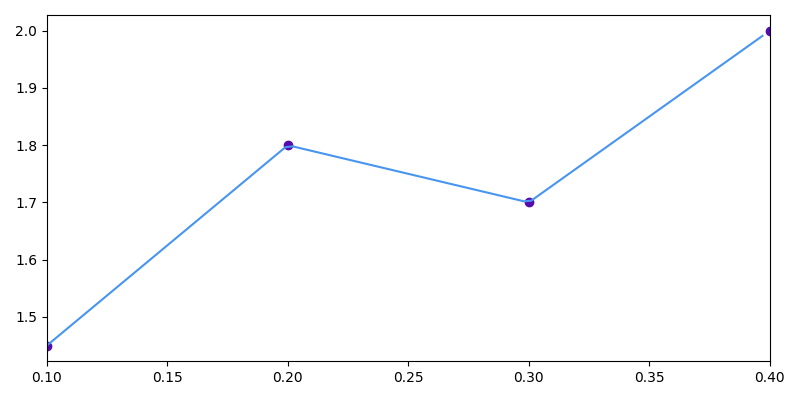
\includegraphics[width=14 cm]{Graphics/problema3.png}
    \caption{Spline de grado 1 usando los puntos $\{(0.1,1.45) ,(0.2,1.8), (0.3,1.7),( 0.4,2.0)\}$.}
    \label{fig:problema3}
\end{figure}

\pagebreak